\documentclass [12pt, titlepage]{article}

\usepackage[margin=1in]{geometry}
\usepackage[all]{nowidow}
\usepackage[
    citestyle=authortitle,
    autocite=footnote
]{biblatex}
    \addbibresource{bibliography.bib}
\usepackage{float}
\usepackage{amsfonts}
\usepackage{amssymb}
\usepackage{amsmath}
    \numberwithin{equation}{section}
\usepackage{amsthm}
    \newtheorem{theorem}{Theorem}
    \newtheorem*{definition}{Definition}
\usepackage[
    colorlinks,
    linkcolor=black,
    citecolor=black,
    urlcolor=blue
]{hyperref}
\usepackage{graphicx}
    \graphicspath{{media/}} 
\usepackage{mdframed}
\usepackage{pgfplots}
\usepackage{caption}
\usepackage{nicefrac}

\setlength{\parskip}{1em}
\setlength{\parindent}{0em}

\let\oldsection\section
\renewcommand\section{\clearpage\oldsection}

\renewcommand{\geq}{\geqslant}
\renewcommand{\Re}{\text{Re}}
\renewcommand{\Im}{\text{Im}}
\newcommand{\ahalf}{\frac{1}{2}}

% commonly used integrals
\newcommand{\piint}{\int_{-\pi}^{\pi}} % -pi to pi
\newcommand{\infint}{\int_{-\infty}^{\infty}} % -infinity to infinity

\title{How can a tiny mp3 player store thousands of songs}
\author{Michalis Pardalos}
\date{}

\begin{document}
\maketitle
\tableofcontents

\section{Introduction}
\section{The Fourier Series}

The Fourier Series is defined as a series of the form
%
\begin{equation} \label{eq:fourier_series}
    f(t) = a_0 + \sum_{n=1}^{\infty}a_n \cos{nt} + \sum_{n=1}^{\infty}b_n \sin{nt}
\end{equation}
%
where $a_n$, $b_n$ constants. 

\subsection{Finding the coefficients} \label{sec:fourier_coefficients}

Before explaining how the Fourier coefficients are found, it will help to state the
following integral identities\autocite[438]{courant_calculus_1}.
%
\begin{align}
    \piint \sin{nx}\ dx          & = 0 \label{eq:sinint}\\
    \piint \cos{nx}\ dx          & = 0 \label{eq:cosint}\\
    \piint \sin{nx}\cos{mx}\ dx & = 0\label{eq:sincosint}\\
    \piint \cos{nx}\cos{mx}\ dx & =
    \begin{cases}
        0,   & m\not=n\\
        \pi, & m=n
    \end{cases} \label{eq:coscosint}\\
    \piint \sin{nx}\sin{mx}\ dx &= 
    \begin{cases}
        0,   & m\not=n\\
        \pi, & m=n\not=0
    \end{cases} \label{eq:sinsinint}
\end{align}
%
With these in mind, we can begin with finding some coefficients for the Fourier expansion of
a function $f(t)$. It is assumed \textbf{that the period of $f(t)$ is
$2\pi$ and that it is symmetric about $x=0$}, this means that the interval $[-\pi, \pi]$,
covers exactly one complete period of $f(t)$:
%
\begin{equation*}
    f(t) = a_0 + \sum_{n=1}^\infty a_n \cos{nt} + \sum_{n=1}^{\infty} b_n \sin{nt}
\end{equation*}
%

First we can find $a_0$ simply by integrating with respect to $t$ over $[-\pi, \pi]$:
%
\begin{equation*}
    \piint f(t)\ dt = a_0\piint dt + \sum_{n=1}^\infty a_n \piint \cos{nt}\ dt 
        + \sum_{n=1}^{\infty} b_n \piint \sin{nt}\ dt\\
\end{equation*}
%
By equations \eqref{eq:sinint} and \eqref{eq:cosint}, this can be simplified to:
%
\begin{equation*}
    \piint f(t)\ dt &= 2\pi a_0\\
\end{equation*}
%
So, $a_0$ can be found as:
%
\begin{mdframed}
    \begin{equation}
        a_0 &= \frac{1}{2\pi}\piint f(t)\ dt
    \end{equation}
\end{mdframed}
%

Next, for $a_n$, say we want to find some $a_m$. Multiplying by $\cos{mt}$ and integrating
with respect to $t$ over $[-\pi, \pi]$ gives us:
%
\begin{equation*}
    \piint f(t)\cos{mt}\ dt =  a_0\piint \cos{mt}\ dt 
        + \sum_{n=1}^\infty a_n \piint \cos{nt}\cos{mt}\ dt 
        + \sum_{n=1}^{\infty} b_n \piint \sin{nt}\cos{mt}\ dt
\end{equation*}
%
Using equations \eqref{eq:cosint}, \eqref{eq:sincosint} and \eqref{eq:coscosint} this is reduced to:
%
\begin{equation*}
    \piint f(t)\cos{mt}\ dt = \pi a_m
\end{equation*}
%
So, any given $a_m$ can be found as:
%
\begin{mdframed}
    \begin{equation}
        a_m = \frac{1}{\pi}\piint f(t)\cos{mt}\ dt
    \end{equation}
\end{mdframed}
%

Similarly, to find some $b_m$, $m > 0$, we can multiply $f(t)$ by $\sin{mt}$ and integrate
with respect to $t$ over $[-\pi, \pi]$ to get:
%
\begin{equation*}
    \piint f(t)\sin{mt}\ dt = a_0\piint \sin{mt}\ dt 
        + \sum_{n=1}^\infty a_n \piint \cos{nt}\sin{mt}\ dt 
        + b_n \piint \sin{nt}\sin{mt}\ dt
\end{equation*}
%
Using equations \eqref{eq:sinint}, \eqref{eq:sincosint} and \eqref{eq:sinsinint}, we can see
that
%
\begin{mdframed}
    \begin{equation}
        b_m = \frac{1}{\pi}\piint f(t)\sin{mt}\ dt
    \end{equation}
\end{mdframed}

\subsection{Simplifying the Series using Euler's Formula}

While the coefficients are relatively simple to find once someone has the formulas in
\autoref{sec:fourier_coefficients}, it is often cumbersome to find 3 coefficients. We can
simplify the series to use just one coefficient using Euler's Formula.

Euler's Formula states that
%
\begin{equation} \label{eq:euler}
    e^{ix} = \cos{x} + i\sin{x}
\end{equation}
%
This can also be restated as 
%
\begin{equation} \label{eq:neg_euler}
    e^{-ix} = \cos{x} - i\sin{x}
\end{equation}
%
Adding or subtracting equations \eqref{eq:euler} and \eqref{eq:neg_euler} gives,
respectively:
%
\begin{align*}
    \cos{x} &= \frac{e^{ix} + e^{-ix}}{2} \label{eq:euler_cos}\\ 
    \sin{x} &= \frac{e^{ix} - e^{-ix}}{2i} \label{eq:euler_sin}
\end{align*}
%

Using these formulas, the Fourier series --- as stated in \autoref{eq:fourier_series}---
becomes:
%
\begin{equation*}
    f(t) &= a_0 + \sum_{n=1}^\infty a_n\frac{e^{int} + e^{-int}}{2} 
            + \sum_{n=1}^\infty b_n \frac{e^{int} - e^{-int}}{2i} 
\end{equation*}
%
It will make the calculations easier at this point to combine the sums. First, note that
$\frac{e^{int}+e^{-int}}{2} = 1$ for $n=0$. $a_0$ can therefore be added into the first sum,
by having it start from $n=0$. Also note that $\frac{e^{int}-e^{-int}}{2i} = 0$ for $n=0$,
so starting the second sum from $0$ does not affect the series. We can therefore combine the
series into a single sum.
%
\begin{align}
    f(t) &= \sum_{n=0}^{\infty} a_n\frac{e^{int} + e^{-int}}{2} 
            + b_n \frac{e^{int} - e^{-int}}{2i} \nonumber \\
         &= \sum_{n=0}^\infty \frac{a_n}{2}e^{int} + \frac{a_n}{2} e^{-int} 
            + \frac{b_n}{2i}e^{int} - \frac{b_n}{2i}e^{-int} \nonumber\\
         &= \sum_{n=0}^\infty \frac{a_n}{2} e^{int} + \frac{a_n}{2} e^{-int} 
            - \frac{b_n}{2} ie^{int} + \frac{b_n}{2} ie^{-int} \nonumber\\
         &= \sum_{n=0}^\infty \ahalf(a_n - ib_n)e^{int} + \ahalf(a_n + ib_n)e^{-int}
            \label{eq:complex_fourier_halfway}
\end{align}
%
Notice, that the two coefficients $a_n + ib_n$ and $a_n - ib_n$ are conjugates of each
other. We can, therefore, define a new constant $c_n$, to replace $a_n$ and $b_n$:
\autocite{fourier_lecture}
%
\begin{equation*}
    c_n = 
    \begin{cases}
        \ahalf \left(a_n - ib_n \right)        & n \geq 0\\
        \ahalf \left(a_{|n|} + ib_{|n|}\right) & n < 0
    \end{cases}
\end{equation*}
%
With this definition, continuing from \eqref{eq:complex_fourier_halfway}, we can restate
the series as:
%
\begin{equation} \label{eq:complex_fourier}
    f(t) = \sum_{n=-\infty}^{\infty}c_n e^{int}
\end{equation}
%
In this form, the series is referred to as the \emph{complex Fourier series}.

We can substitute the formulas for $a_n$ and $b_n$ into the cases for $c_n$ to obtain a
singular formula for it. Let us begin with the case of $n \geq 0$
%
\begin{align}
    c_n &= \ahalf(a_n - ib_n) \nonumber \\
        &= \ahalf \left(\frac{1}{\pi} \piint f(t)\cos{nt}\ dt 
            - i\frac{1}{\pi}\piint f(t)\sin{nt}\ dt \right) \nonumber \\
        &= \frac{1}{2\pi}\piint f(t) (\cos{nt} - i\sin{nt})\ dt \nonumber \\
        &= \frac{1}{2\pi}\piint f(t) e^{-int}\ dt \label{eq:c_n_pos_euler}
\end{align}
%

Similarly, for $n < 0$:
%
\begin{align}
    c_n &= \ahalf(a_{|n|} + ib_{|n|}) \nonumber \\
        &= \ahalf \left(\frac{1}{\pi} \piint f(t)\cos{|n|t}\ dt 
            + i\frac{1}{\pi}\piint f(t)\sin{|n|t}\ dt \right) \nonumber \\
        &= \frac{1}{2\pi}\piint f(t) (\cos{|n|t} + i\sin{|n|t})\ dt \nonumber \\
        &= \frac{1}{2\pi}\piint f(t) e^{i|n|t}\ dt \nonumber \\
        &= \frac{1}{2\pi}\piint f(t) e^{-int}\ dt & \text{Since }n<0 \label{eq:c_n_neg_euler}
\end{align}
%
Since the formulas \eqref{eq:c_n_pos_euler} and \eqref{eq:c_n_neg_euler} are the same, we
can say for all $n \in \mathbb{Z}$:
\begin{mdframed}
    \begin{equation*}
        c_n = \frac{1}{2\pi}\piint f(t) e^{-int}\ dt
    \end{equation*}
\end{mdframed}


\section{The Fourier Transform}

The Fourier Transform is the extension of the Fourier Series for functions defined in all of
$-\infty < x < \infty$, and for non-integer frequencies of sinusoids. There are two
operations related to the Fourier Transform: The Forward Fourier Transform and the Inverse
Fourier Transform. The former is analogous to $c_n$ for the Fourier Series, giving the
amplitude of the sinusoid of frequency $u$ in $f$, with the difference being, that $u$ can
take non-integer values, contrary to $n$ which is a discrete variable. In relation to the
Fourier Series, the Fourier Transform can be thought of as its limit as the period of the
function being approximated approaches infinity.  \autocite{wolfram_fourier_transform} 

The Fourier Transform of a function can be thought of as an alternative represantation of
a function. It holds the exact same information as the the original function, but presents
it in a different way, which is often more useful than the original representation. If a
function is thought of as a signal that varies over time, then its Fourier Transform is a
representation of the base frequencies that make it up, 

The formulas for the Fourier Transform and its inverse can be seen below:
%
\begin{align*}
    F(u) &= \infint f(t)e^{-2\pi itu}\ dt && \text{(Forward Fourier Transform)}\\[1em]
    f(t) &= \infint F(u)e^{2\pi itu}\ du && \text{(Inverse Fourier Transform)}
\end{align*}
%

As an example, here is the Fourier Transform for a square pulse, a function which has a
constant value between two bounds, and is zero everywhere else, i.e.
%
\begin{equation*}
    f(x) = \begin{cases}
        A &a < x < b\\
        0 &\text{otherwise}
    \end{cases}:\ A,a,b \in \mathbb{R}
\end{equation*}
%
For the example, I will use a square pulse from $-\pi$ to $\pi$ of height 2
(\autoref{fig:square_pulse}).
%
\begin{figure}[H]
    \centering
    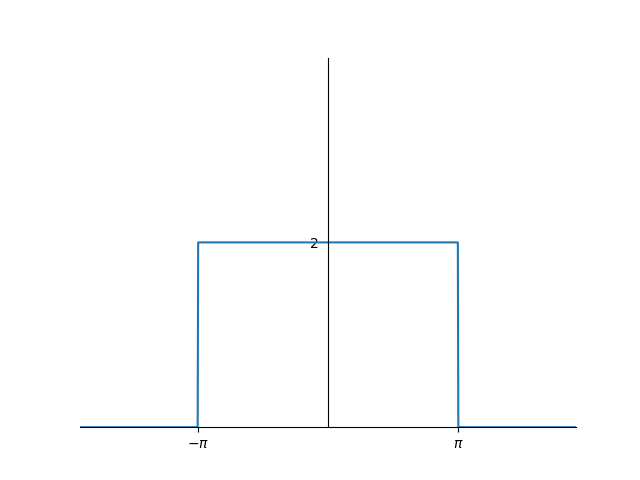
\includegraphics[width=.6\textwidth]{square_pulse}
    \caption{}
    \label{fig:square_pulse}
\end{figure}
%
Taking its Fourier Transform:
%
\begin{equation*}
    F(u) =  \infint f(t) e^{-2\pi itu}\ dt
\end{equation*}
%
It becomes clear that the only interval that matters is $[-\pi, \pi]$. So the integral
becomes:
%
\begin{equation*}
    F(t) = \piint f(t)e^{-2\pi itu}\ dt
\end{equation*}
%
But, $f(t)$ has a constant value of $2$ in that interval. So, again, the integral is
simplified to:
%
\begin{equation*}
    F(t) &= 2 \piint e^{-2\pi itu}\ dt
\end{equation*}
%
Then, it is simply a matter of finding the antiderivative and integrating:
%
\begingroup
\addtolength{\jot}{1em}
\begin{align*}
    F(u) &= \frac{2}{-2\pi iu} \piint -2\pi iue^{-2\pi itu}\ dt \\
         &= \frac{1}{-\pi iu} \left[e^{-2\pi itu}\right]_{-\pi}^{\pi}\\
         &= \frac{e^{-i2\pi^{2}u} - e^{i2\pi^{2}u}}{-\pi iu}\\
         &= \frac{-2i\sin{(2\pi^{2}u)}}{-\pi iu}\\
         &= \frac{2\sin{(2\pi^{2}u)}}{\pi u}
\end{align*}
\endgroup
%

\autoref{fig:ft_of_square_pulse} shows the plot of this function.
\begin{figure}[H]
    \centering
    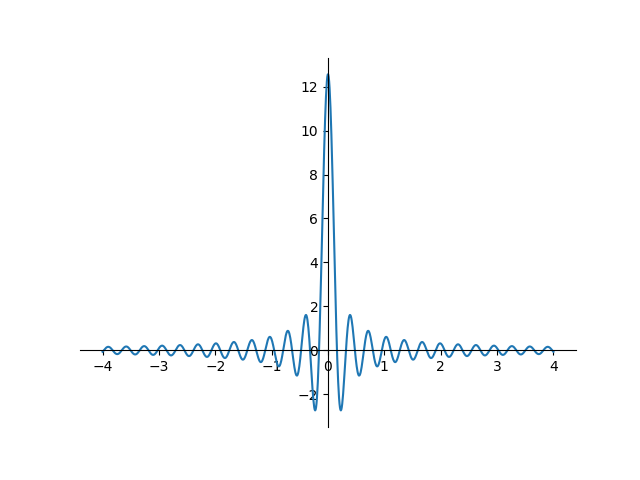
\includegraphics[width=.6\textwidth]{ft_of_square_pulse}
    \caption{}
    \label{fig:ft_of_square_pulse}
\end{figure}


\section{The Discrete Fourier Transform}

The Fourier Transform is extremely useful and has a variety of applications, but it comes
with a crucial limitation: it requires a well-defined, smooth function.
\autocite[319]{courant_calculus_2} In real world applications, however, it is often the case
that one has to obtain the Fourier Transform for a function which is only defined as a set
of points. This means that it is impossible to obtain the Fourier Transform using its
integral formula ($F(u) = \infint f(t) e^{-2\pi itu}\ dt$). 

In this case, the \emph{Discrete Fourier Transform} --- or DFT --- is used. The DFT provides
the base frequencies for a discrete set of data. 

For a discrete set of $N$ points labelled $f_k$ where $k \in \mathbb{Z}$ and $k \in [0,
N-1]$, the DFT can be obtained by considering a function $f(k)$ which has an area of $f_k$
where $k \in \mathbb{Z}$ and $k \in [0, N-1]$, and 0 everywhere else. Then, the Fourier
Transform Integral can be computed as a sum. Since there is only $N$, discrete, inputs to the
transform, only $N$, discrete, outputs will be meaningful. So, for $n \in [0, N-1]$, the
Fourier Transform of $f_k$ is:
%
\begin{equation}
    F_n = \sum_{k=0}^{N-1} f_k e^{-2\pi ikn / N}
\end{equation}
%
Similarly, the Inverse Fourier Transform is:
%
\begin{equation}
    f_k = \frac{1}{N} \sum_{n=0}^{N-1} F_n e^{2\pi ikn / N}
\end{equation}
%

The Discrete Fourier Transform is also especially practical because of an extremely
efficient algorithm for computing it appropriatelly called the \emph{Fast Fourier Transform}
--- or \emph{FFT} --- 
    
\section{The Fourier Transform in MP3 compression}

MPEG-1 layer 3, better known as MP3, is the most widely used standard for electronically
encoding audio. It has achieved this level of popularity mainly because of the very small
size of the files that are produced when audio is encoded using it. This is largely due to
its use of the (Discrete) Fourier Transform. \autocite{mp3_paper}

The first step of the algorithm is breaking up the audio into so called frames. The
compression algorithm is applied to each frame separately.

Because MP3 belongs to a family of compression algorithms called \emph{lossy} compression
algorithms, which do not retain all input data. They ignore data that can be removed with
small effects on the output. In the case of MP3 --- and lossy audio compression in general
--- this means removing certain frequencies from the audio. 

A Discrete Fourier Transform is first applied to the audio. The number of samples used for
it depends on the \emph{bitrate} chosen for the encoding. Bitrate is the measure of how many
bytes of data are used for each second of the audio, and can have a value of up to 320
kilobytes per second in MP3. The DFT gives the base frequencies present in the frame. Then
the \emph{psychoacoustic model} is applied on the data. This model is a way of determining
frequencies that will least affect the experience of the listener. The first, most obvious
step is removing frequencies that are completely inaudible to the human ear, namely anything
under 20Hz or over 20kHz. The most important optimization, however, relies on the fact that
frequencies close to another, very strong one are \emph{"masked"}, meaning that their impact
is lessened. The strength of this masking effect is smoothly reduced as frequencies get
further away from the very strong frequency. This effect is used by creating a cutoff
threshold around the very strong frequencies. Frequencies below the threshold value are
not included in the final file. 

The MP3 standard includes a number of other parts and ways of reducing file size. The
primary part of the encoding is still the psychoacoustic model however, and so other parts
of the encoding are outside the scope of the investigation.

\printbibliography
\end{document}
